\documentclass[aspectratio=169]{beamer}


%-------------------------------------------------------
% USED PACKAGES
%-------------------------------------------------------
\usepackage{packages}

%-------------------------------------------------------
% OVERALL TEMPLATE
%-------------------------------------------------------
\usetheme[]{Feather}

%-------------------------------------------------------
% LAYOUT OF THE TITLE PAGE
%-------------------------------------------------------
\usepackage{title}


\usepackage{style}

%-------------------------------------------------------
% COLOURS, MATH OPERATORS,...
%-------------------------------------------------------
\usepackage{command}

%-------------------------------------------------------
% ENVIRONMENTS
%-------------------------------------------------------
\usepackage{theorem}
\setbeamertemplate{frametitle continuation}[from second]

%-------------------------------------------------------
% INFORMATION IN THE TITLE PAGE
%-------------------------------------------------------
\usepackage{title_information}

%-------------------------------------------------------
% THE BODY OF THE PRESENTATION
%-------------------------------------------------------

\begin{document}
%-------------------------------------------------------
% THE TITLEPAGE
%-------------------------------------------------------
\begin{frame}[plain,noframenumbering] % the plain option removes the header from the title page, noframenumbering removes the numbering of this frame only
  \titlepage % call the title page information from above
\end{frame}

\AtBeginSection[]{
\begin{frame}[noframenumbering]{Contents}
\setcounter{tocdepth}{2}
\tableofcontents[sectionstyle=show/shaded, subsectionstyle=show/show/hide]
\end{frame}
}

\begin{frame}{Contents}
\setcounter{tocdepth}{2}
\tableofcontents
\end{frame}
%
%-------------------------------------------------------
\section{MSI spatial distribution: a proposal for modelling}
%-------------------------------------------------------
\subsection{General framework}
\begin{frame}{General framework}{The sample distribution}
%	\begin{itemize}
%		\item \underline{The sample:} $M = (M_{1}, \hdots, M_{n})$ consisting of $n$ entities;
%		\item \underline{The sample locations:} $X = (X_{1}, \hdots, X_{n})$ (where the entities are located);
%		\item \underline{The location distribution:} $f_{X}$ the random mechanism ruling the spatial spread;
%	\end{itemize}
	\begin{figure}[H]
		\label{mapping1}\caption{Spatial distribution $f_{X}$ in $m^{-2}$ and a sample $(X_{1}, \hdots, X_{n})$ from it}
		\centering
    	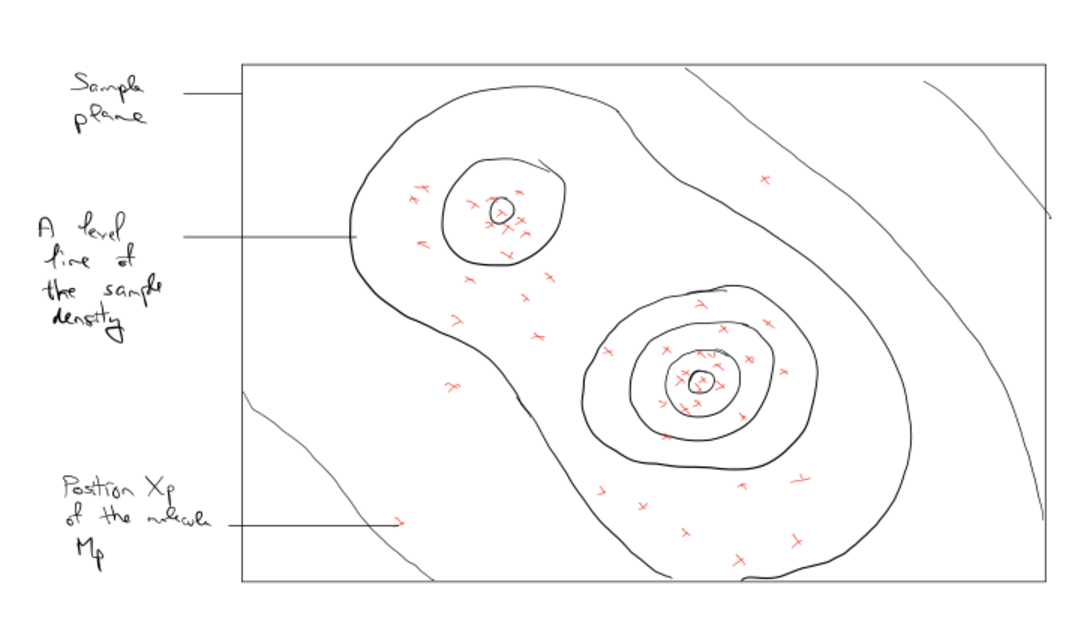
\includegraphics[scale = .5, keepaspectratio]{modelling/general/sample_distribution.pdf}
	\end{figure}
\end{frame}

\begin{frame}{General framework}{The sampling design}
\begin{itemize}
\item \underline{Discrete sampling:} the laser stops at $q$ different spots $(y_{1}, \hdots, y_{q})$ for a fixed duration $t_{0}$;
\item \underline{Continuous sampling:} the laser is driven along a path $\Gamma$ and its position at time $t$ is $\Gamma(t)$;
\end{itemize}

\begin{columns}[c]
	\begin{column}{5.75cm}
			\begin{figure}[H]
		\label{mapping1}\caption{Sampling design $(y_{1}, \hdots, y_{q})$ in spot mode}
		\centering
    	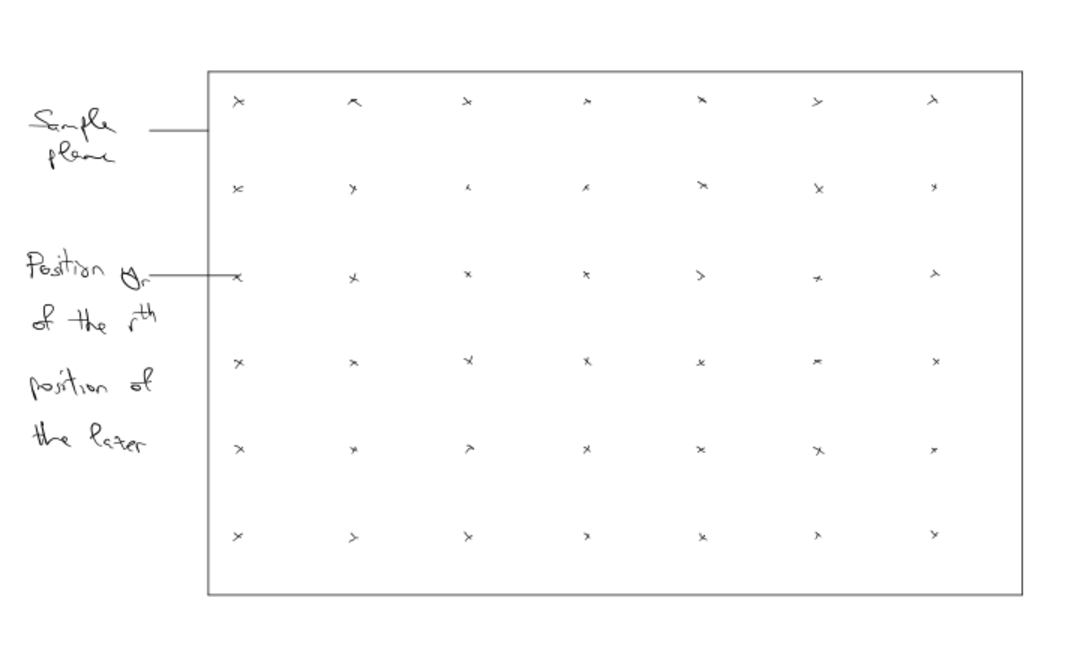
\includegraphics[width=\textwidth,height=\textheight,keepaspectratio]{modelling/general/sampling_design1.pdf}
	\end{figure}
	\end{column}
	\begin{column}{5.75cm}
			\begin{figure}[H]
		\label{mapping1}\caption{Sampling design $\Gamma$ in raster mode}
		\centering
    	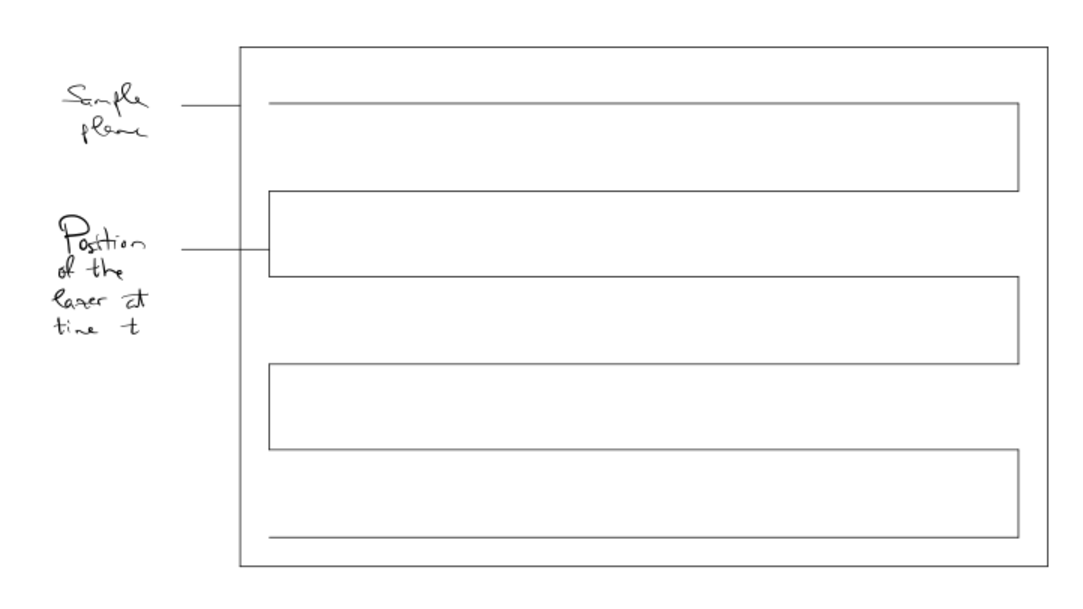
\includegraphics[width=\textwidth,height=\textheight,keepaspectratio]{modelling/general/sampling_design2.pdf}
	\end{figure}
	\end{column}
\end{columns}
\end{frame}

\begin{frame}{General framework}{The ionisation phenomenon I}
\begin{columns}[c]
	\begin{column}{5.75cm}
			\begin{figure}[H]
		\label{mapping1}\caption{Laser irradiance $I(x)$ in $W.m^{-2}$}
		\centering
    	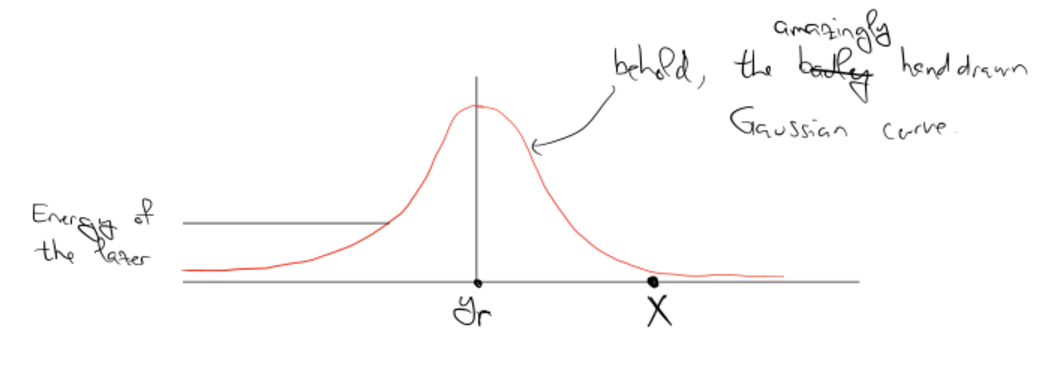
\includegraphics[width=\textwidth,height=\textheight,keepaspectratio]{modelling/general/ionisation1.pdf}
	\end{figure}
	\end{column}
	\begin{column}{5.75cm}
			\begin{figure}[H]
		\label{mapping1}\caption{Ionisation probability function $\mathcal{I}_{\mathds{P}}(t, y_{r} - X)$}
		\centering
    	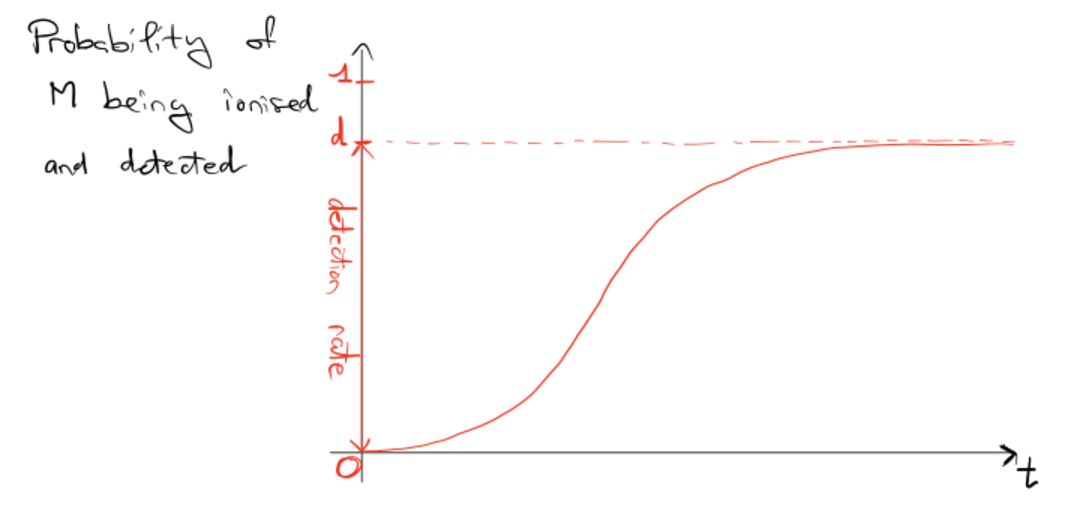
\includegraphics[width=\textwidth,height=\textheight,keepaspectratio]{modelling/general/ionisation2.pdf}
	\end{figure}
	\end{column}
\end{columns}
\end{frame}

\begin{frame}{General framework}{The ionisation phenomenon II}
\begin{figure}[H]
	\label{mapping1}\caption{Ionisation probability function $\mathcal{I}_{\mathds{P}}(t_{0}, y - x)$ for different values of $t_{0}$}
	\centering
    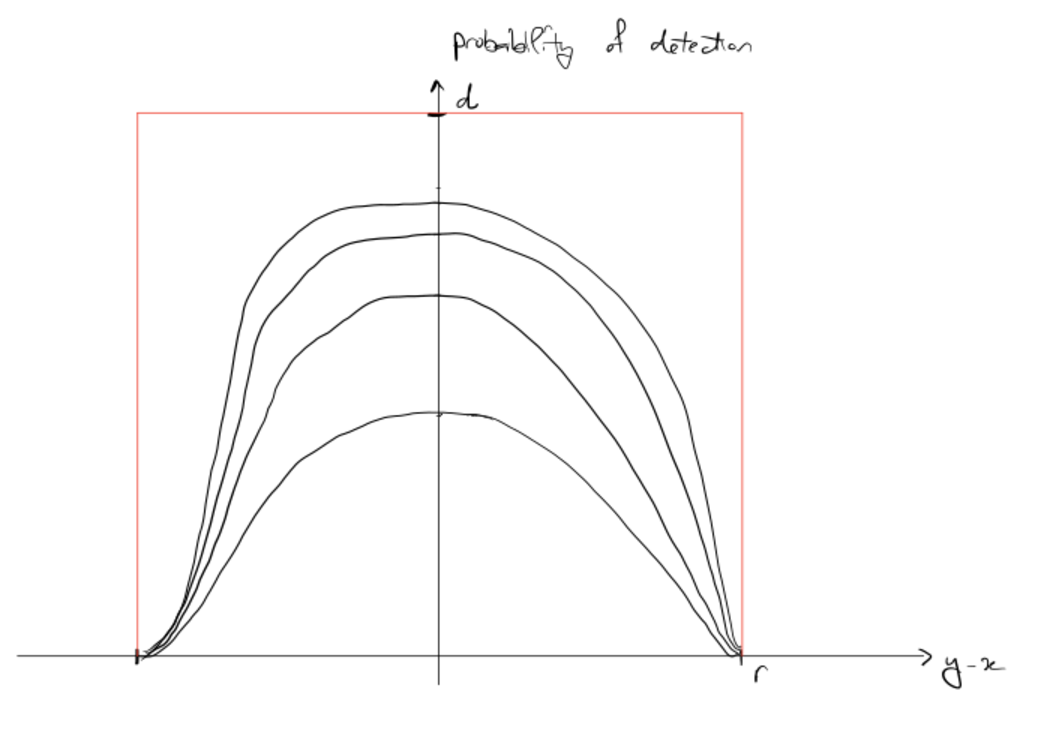
\includegraphics[scale = .45, keepaspectratio]{modelling/general/ionisation3.pdf}
\end{figure}
\end{frame}

\subsection{The (under)sampling case}
%%% MetaPost direct problem inference
\begin{frame}{Oversampling: where will we see the molecule?}
\underline{Recorded position:} $Y$ is the position of the laser when the molecule is detected;

\[\mathds{P}(Y = y_{r}) = (\mathcal{I}_{\mathds{P}}(t_{0}, \cdot) \star f_{x})(y_{r}) \cdot \prod\limits_{s = 1}^{r - 1} \left(1 - \left(\mathcal{I}_{\mathds{P}}(t_{0}, \cdot) \star f_{X}\right)(y_{s})\right)\]

\begin{figure}[H]
	\label{mapping1}\caption{The sampling design}
	\centering
    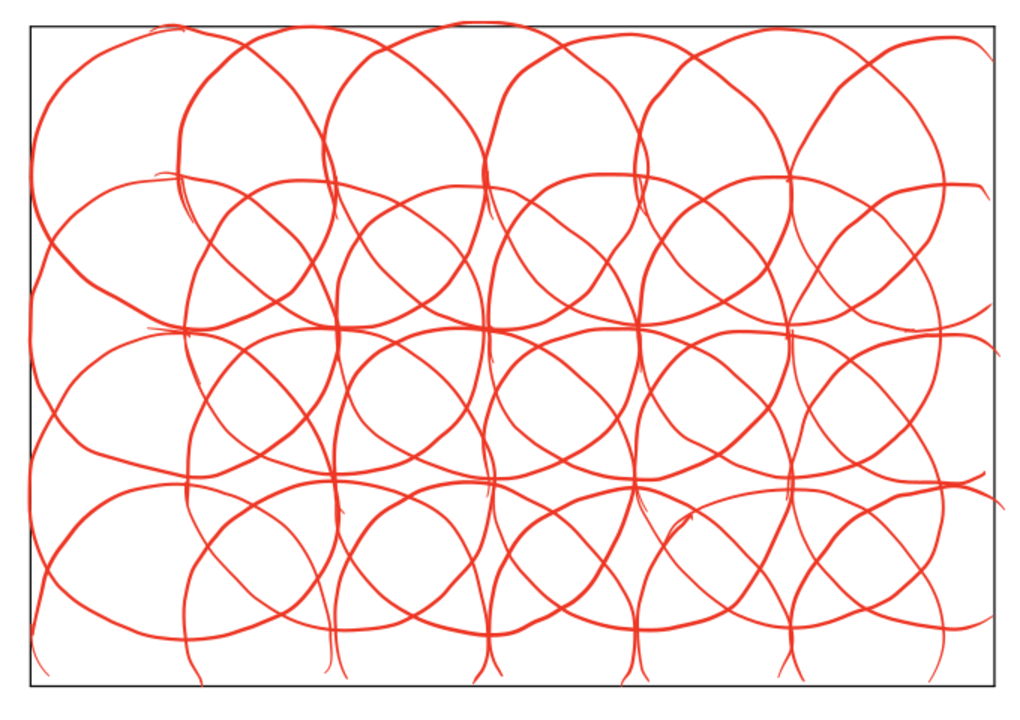
\includegraphics[scale = .3, keepaspectratio]{modelling/oversampling/oversampling.pdf}
\end{figure}

\end{frame}

%% MetaPost Inverse Problem inference
\begin{frame}{The (under)sampling case}{Distribution of the observation}
\underline{Image:}
\begin{itemize}
\item $1$ pixel = $1$ laser position
\item pixel $r$ contains $Z_{r} = \frac{1}{n} \sum\limits_{p = 1}^{n} \mathds{1}_{\{Y_{p} = y_{r}\}}$
\end{itemize}
\[\mathds{P}(Z_{r} = p) = {{n}\choose{n \cdot p}} \cdot \left((\mathcal{I}_{\mathds{P}}(t_{0}, \cdot) \star f_{X})(y_{r})\right)^{n \cdot p} \cdot \left(1 - (\mathcal{I}_{\mathds{P}}(t_{0}, \cdot) \star f_{X})(y_{r})\right)^{n \cdot (1 - p)}\]

\[ \mathds{E}\left[Z_{r}\right] = (\mathcal{I}_{\mathds{P}}(t_{0}, \cdot) \star f_{X})(y_{r}) \]

\[ \mathds{V}\left[Z_{r}\right] \leq \frac{1}{4 \cdot n} \]
\end{frame}

\subsection{The oversampling case}
%%% MetaPost direct problem inference
\begin{frame}{Oversampling: where will we see the molecule?}
\underline{Recorded position:} $Y$ is the position of the laser when the molecule is detected;

\[\mathds{P}(Y = y_{r}) = (\mathcal{I}_{\mathds{P}}(t_{0}, \cdot) \star f_{x})(y_{r}) \cdot \prod\limits_{s = 1}^{r - 1} \left(1 - \left(\mathcal{I}_{\mathds{P}}(t_{0}, \cdot) \star f_{X}\right)(y_{s})\right)\]

\begin{figure}[H]
	\label{mapping1}\caption{The sampling design}
	\centering
    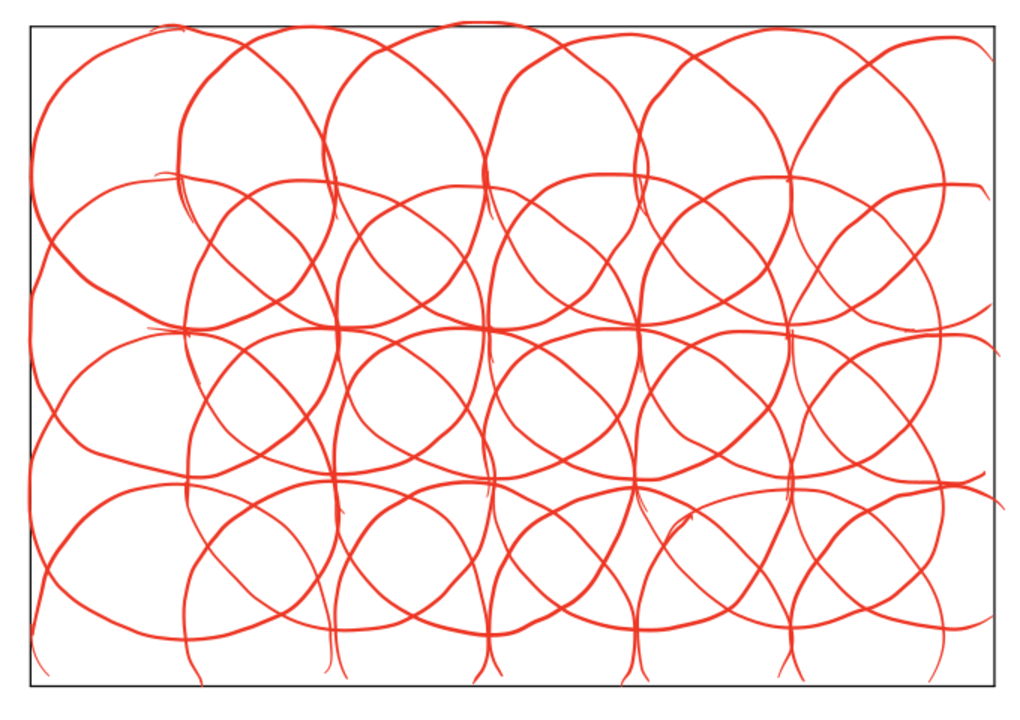
\includegraphics[scale = .3, keepaspectratio]{modelling/oversampling/oversampling.pdf}
\end{figure}

\end{frame}

%% MetaPost Inverse Problem inference
\begin{frame}{The (under)sampling case}{Distribution of the observation}
\underline{Image:}
\begin{itemize}
\item $1$ pixel = $1$ laser position
\item pixel $r$ contains $Z_{r} = \frac{1}{n} \sum\limits_{p = 1}^{n} \mathds{1}_{\{Y_{p} = y_{r}\}}$
\end{itemize}
\[\mathds{P}(Z_{r} = p) = {{n}\choose{n \cdot p}} \cdot \left((\mathcal{I}_{\mathds{P}}(t_{0}, \cdot) \star f_{X})(y_{r})\right)^{n \cdot p} \cdot \left(1 - (\mathcal{I}_{\mathds{P}}(t_{0}, \cdot) \star f_{X})(y_{r})\right)^{n \cdot (1 - p)}\]

\[ \mathds{E}\left[Z_{r}\right] = (\mathcal{I}_{\mathds{P}}(t_{0}, \cdot) \star f_{X})(y_{r}) \]

\[ \mathds{V}\left[Z_{r}\right] \leq \frac{1}{4 \cdot n} \]
\end{frame}
%
%\subsection{Raster mode}
%%%% MetaPost direct problem inference
\begin{frame}{Oversampling: where will we see the molecule?}
\underline{Recorded position:} $Y$ is the position of the laser when the molecule is detected;

\[\mathds{P}(Y = y_{r}) = (\mathcal{I}_{\mathds{P}}(t_{0}, \cdot) \star f_{x})(y_{r}) \cdot \prod\limits_{s = 1}^{r - 1} \left(1 - \left(\mathcal{I}_{\mathds{P}}(t_{0}, \cdot) \star f_{X}\right)(y_{s})\right)\]

\begin{figure}[H]
	\label{mapping1}\caption{The sampling design}
	\centering
    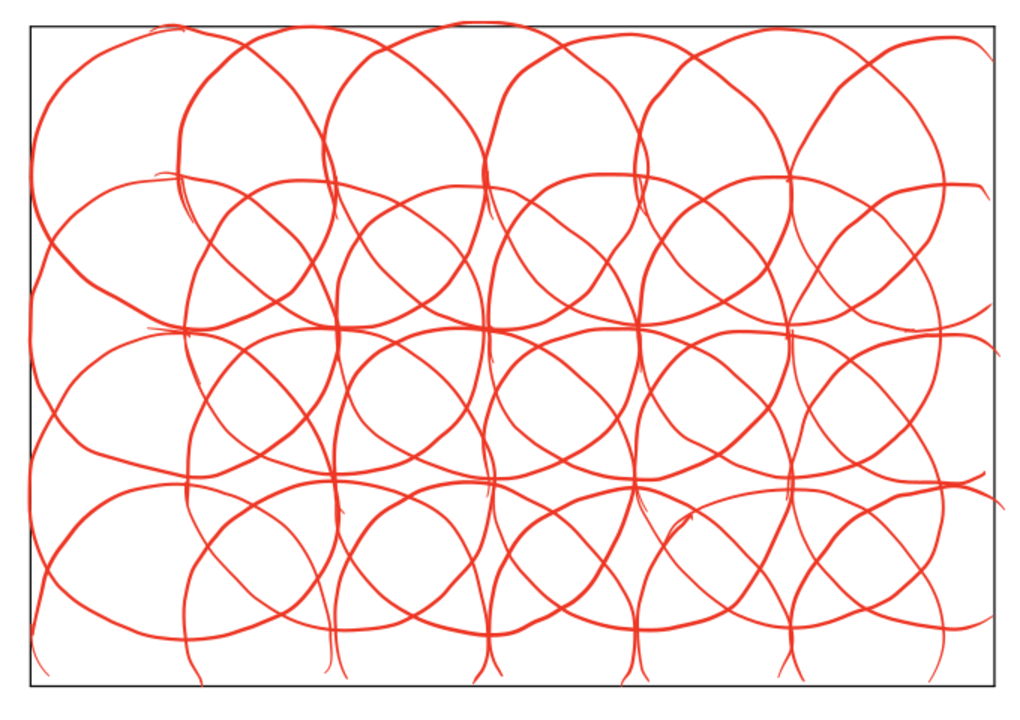
\includegraphics[scale = .3, keepaspectratio]{modelling/oversampling/oversampling.pdf}
\end{figure}

\end{frame}

%% MetaPost Inverse Problem inference
\begin{frame}{The (under)sampling case}{Distribution of the observation}
\underline{Image:}
\begin{itemize}
\item $1$ pixel = $1$ laser position
\item pixel $r$ contains $Z_{r} = \frac{1}{n} \sum\limits_{p = 1}^{n} \mathds{1}_{\{Y_{p} = y_{r}\}}$
\end{itemize}
\[\mathds{P}(Z_{r} = p) = {{n}\choose{n \cdot p}} \cdot \left((\mathcal{I}_{\mathds{P}}(t_{0}, \cdot) \star f_{X})(y_{r})\right)^{n \cdot p} \cdot \left(1 - (\mathcal{I}_{\mathds{P}}(t_{0}, \cdot) \star f_{X})(y_{r})\right)^{n \cdot (1 - p)}\]

\[ \mathds{E}\left[Z_{r}\right] = (\mathcal{I}_{\mathds{P}}(t_{0}, \cdot) \star f_{X})(y_{r}) \]

\[ \mathds{V}\left[Z_{r}\right] \leq \frac{1}{4 \cdot n} \]
\end{frame}

%
%-------------------------------------------------------
\section{What is the point?}
%-------------------------------------------------------
\subsection{Instrument response estimation}
\begin{frame}{Noise estimation}{Data}
\begin{columns}
\begin{column}{8cm}
\begin{figure}[H]
		\label{data_2d}\caption{Data in 2D}
		\centering
    	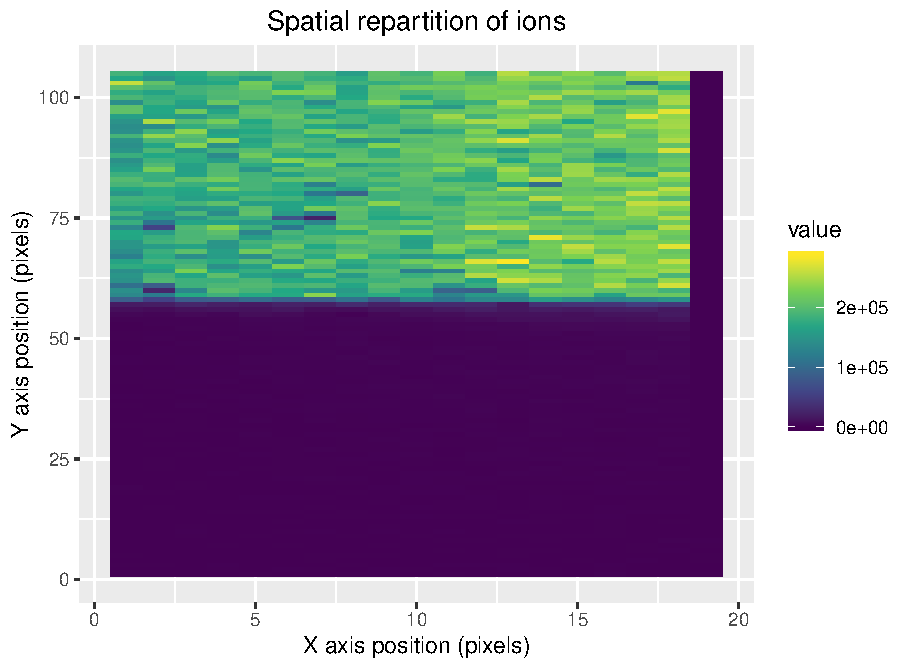
\includegraphics[scale = .5, keepaspectratio]{application/response_estimation/data_2d.pdf}
	\end{figure}
\end{column}
\begin{column}{8cm}
\begin{figure}[H]
		\label{data_1d}\caption{Data in 1D}
		\centering
    	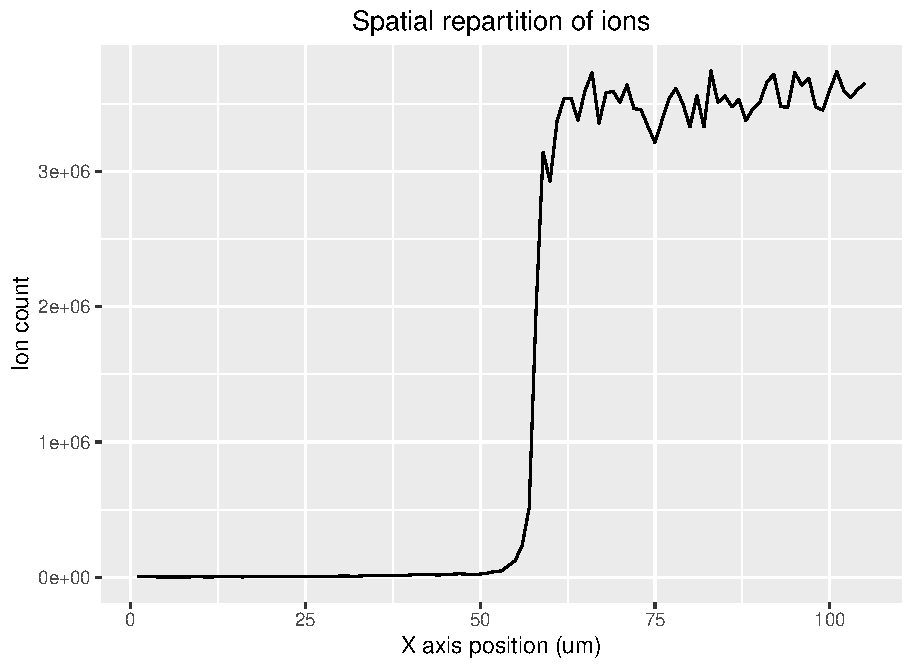
\includegraphics[scale = .5, keepaspectratio]{application/response_estimation/data_1d.pdf}
	\end{figure}
\end{column}
\end{columns}
\end{frame}

\begin{frame}{Noise estimation}{Spectra of data}
\begin{columns}
\begin{column}{8cm}
\begin{figure}[H]
		\label{edge_2d}\caption{Spectra of the data in 2D}
		\centering
    	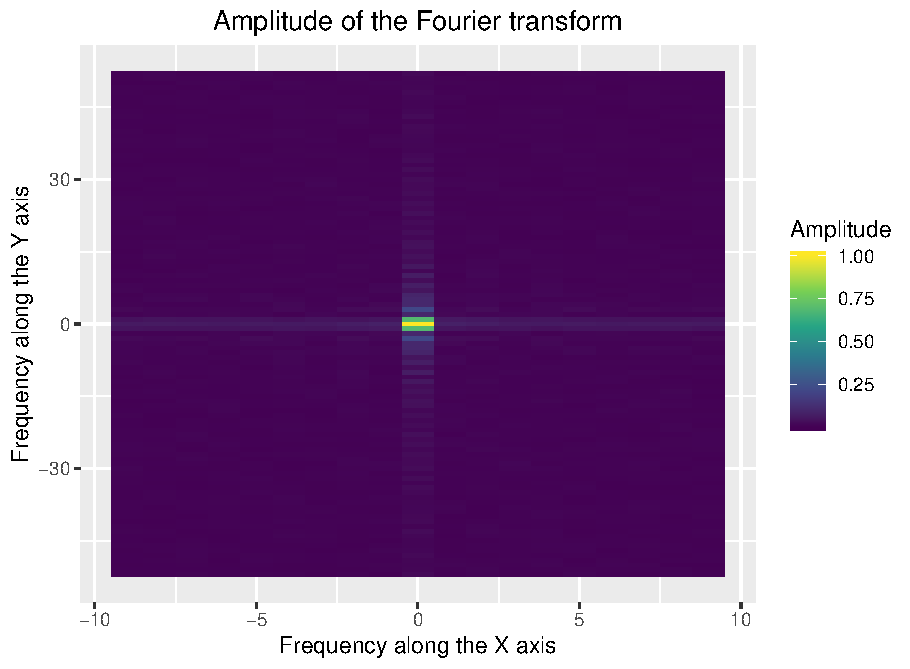
\includegraphics[scale = .5, keepaspectratio]{application/response_estimation/spectra_2d.pdf}
	\end{figure}
\end{column}
\begin{column}{8cm}
\begin{figure}[H]
		\label{edge_2d}\caption{Spectra of the data in 1D}
		\centering
    	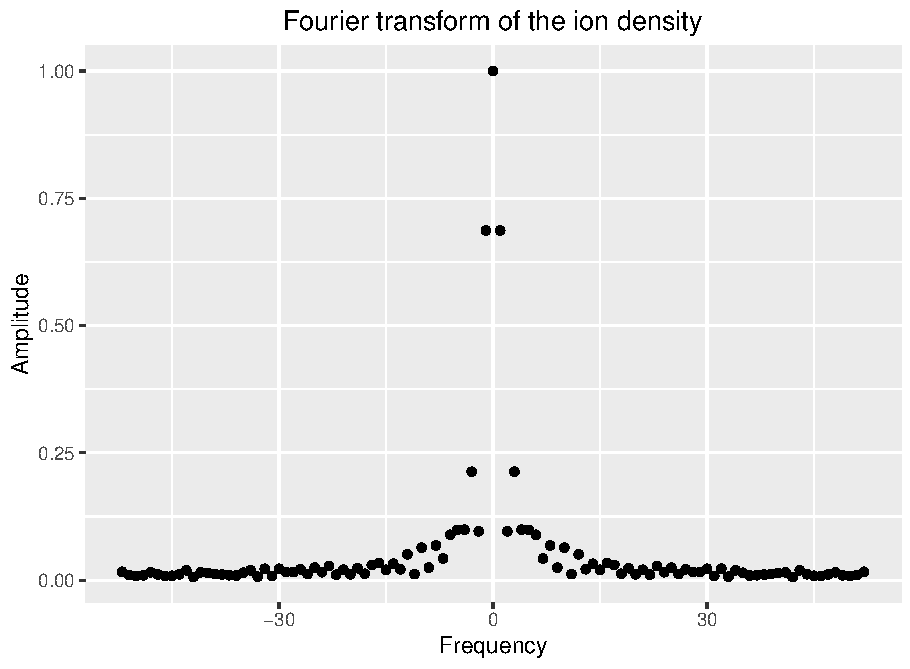
\includegraphics[scale = .5, keepaspectratio]{application/response_estimation/spectra_1d.pdf}
	\end{figure}
\end{column}
\end{columns}
\end{frame}

\begin{frame}{Noise estimation}{Adaptive smoothing as direct problem}
\begin{figure}[H]
		\label{edge_2d}\caption{Adaptive shrinkage estimator in 1D}
		\centering
    	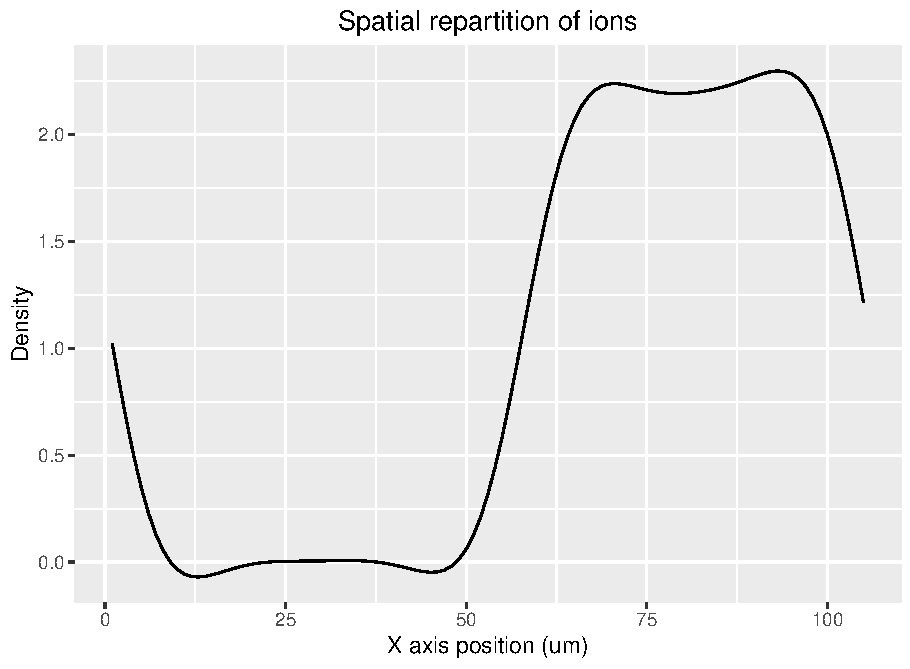
\includegraphics[scale = .5, keepaspectratio]{application/response_estimation/estim_direct_1d.pdf}
	\end{figure}
\end{frame}

\begin{frame}{Noise estimation}{Known distribution of molecules}
\begin{columns}
\begin{column}{8cm}
\begin{figure}[H]
		\label{edge_2d}\caption{Edge in 2D}
		\centering
    	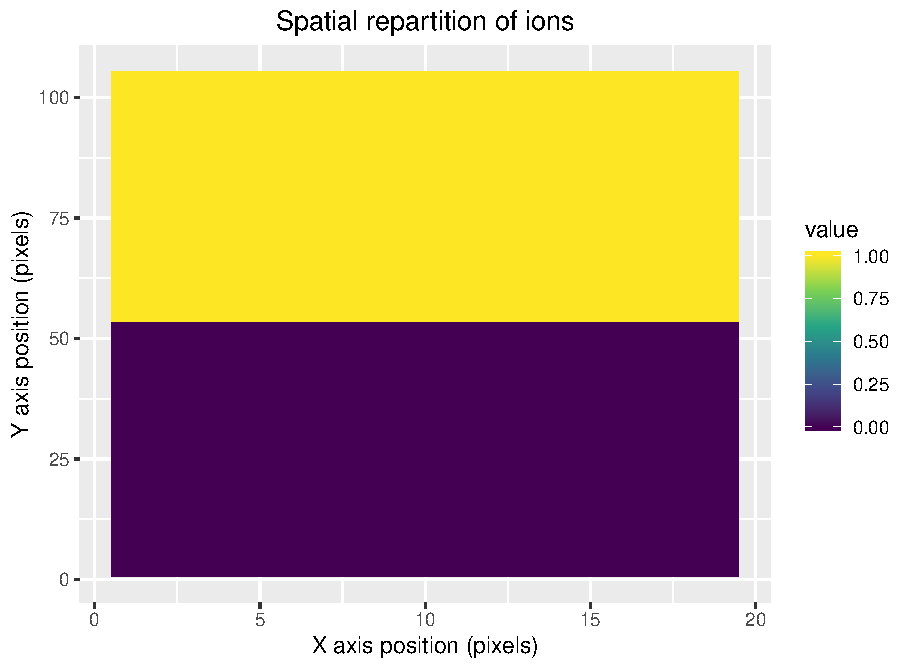
\includegraphics[scale = .5, keepaspectratio]{application/response_estimation/edge_2d.pdf}
	\end{figure}
\end{column}
\begin{column}{8cm}
\begin{figure}[H]
		\label{edge_1d}\caption{Edge in 1D}
		\centering
    	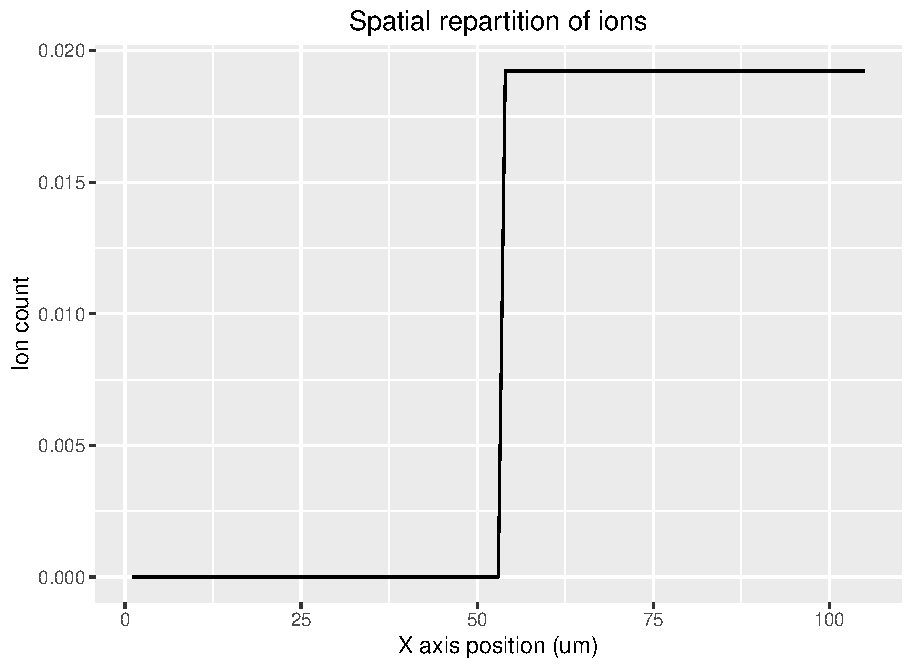
\includegraphics[scale = .5, keepaspectratio]{application/response_estimation/edge_1d.pdf}
	\end{figure}
\end{column}
\end{columns}
\end{frame}

\begin{frame}{Noise estimation}{Spectra of the edge}
\begin{columns}
\begin{column}{8cm}
\begin{figure}[H]
		\label{edge_2d}\caption{Spectra of the edge in 2D}
		\centering
    	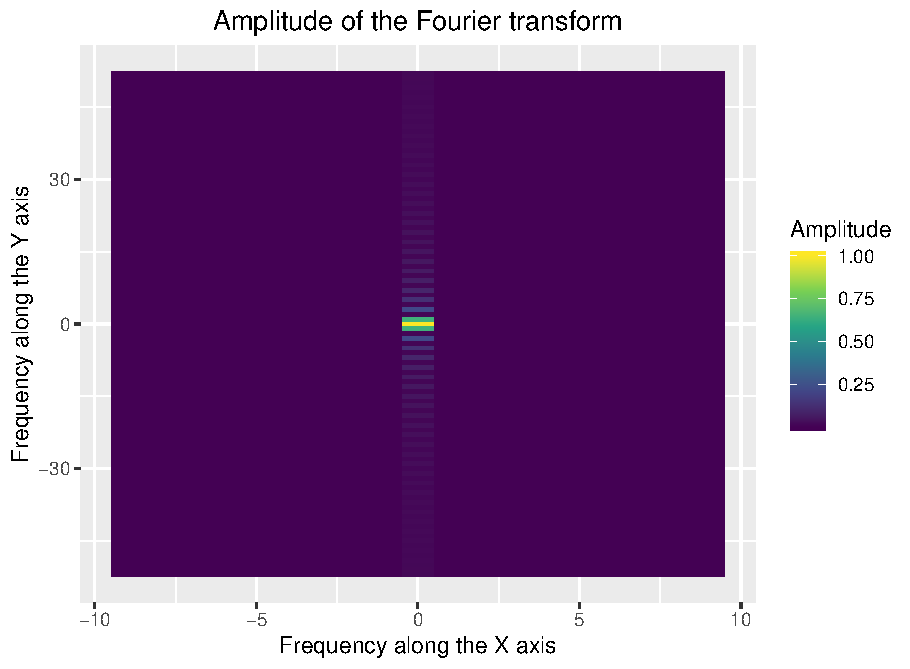
\includegraphics[scale = .5, keepaspectratio]{application/response_estimation/spectra_edge_2d.pdf}
	\end{figure}
\end{column}
\begin{column}{8cm}
\begin{figure}[H]
		\label{edge_2d}\caption{Spectra of the edge in 1D}
		\centering
    	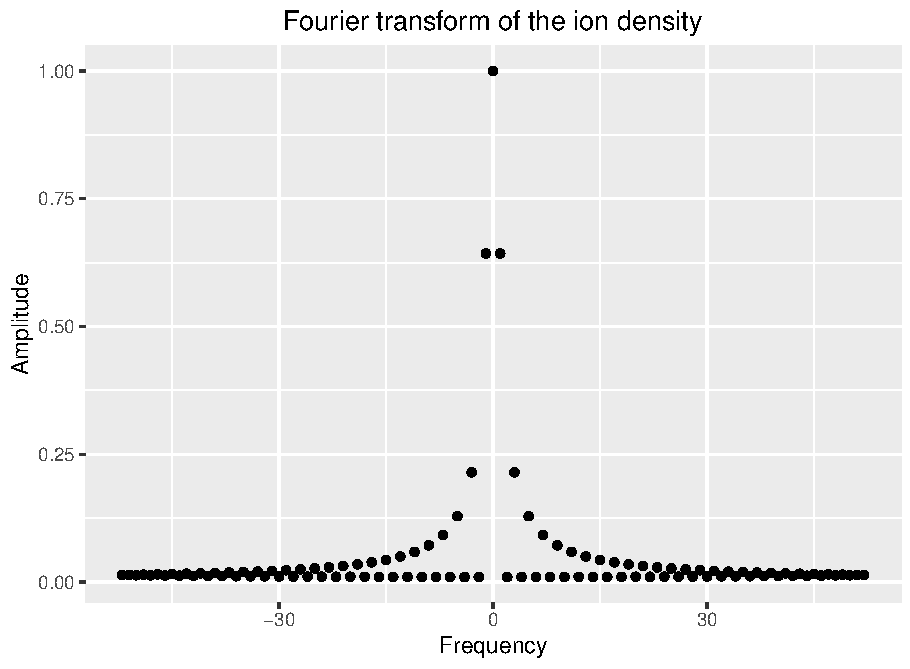
\includegraphics[scale = .5, keepaspectratio]{application/response_estimation/spectra_edge_1d.pdf}
	\end{figure}
\end{column}
\end{columns}
\end{frame}

\begin{frame}{Noise estimation}{Ionisation probability function estimate in 1D}
\begin{columns}
\begin{column}{8cm}
\begin{figure}[H]
		\label{edge_2d}\caption{Adaptive shrinkage estimator of $\mathcal{I}_{\mathds{P}}(t_{0}, \cdot)$ in 1D}
		\centering
    	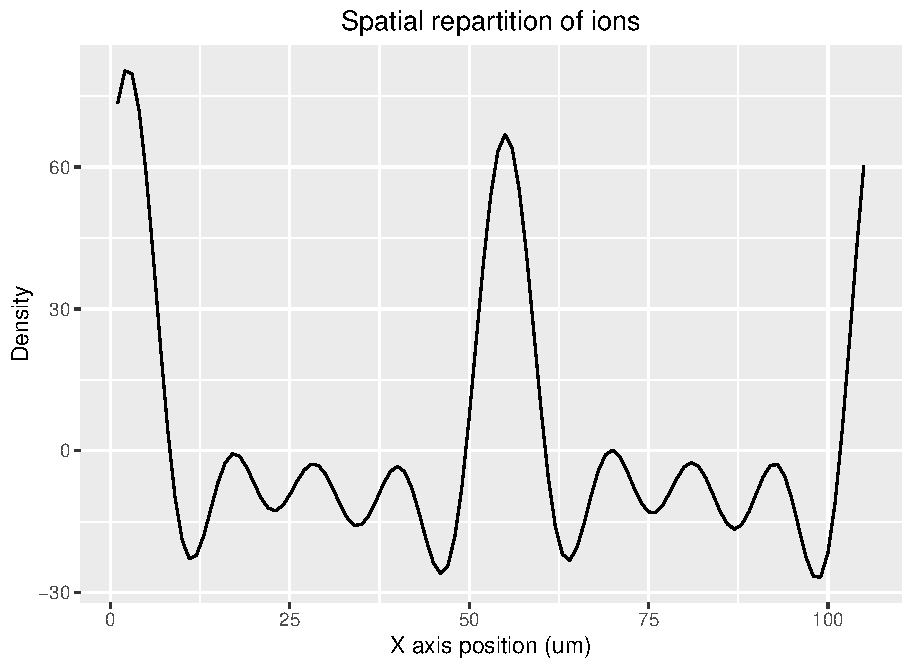
\includegraphics[scale = .5, keepaspectratio]{application/response_estimation/estim_noise_1d.pdf}
	\end{figure}
\end{column}
\begin{column}{8cm}
\begin{figure}[H]
		\label{edge_2d}\caption{Adaptive shrinkage estimator of $\mathcal{I}_{\mathds{P}}(t_{0}, \cdot)$ in 1D}
		\centering
    	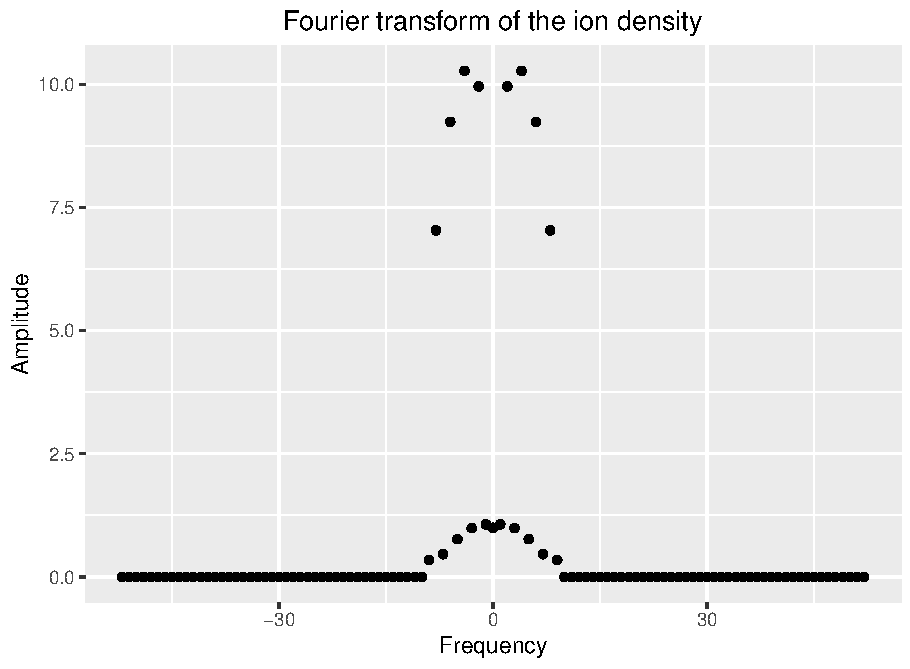
\includegraphics[scale = .5, keepaspectratio]{application/response_estimation/spectra_estim_noise_1d.pdf}
	\end{figure}
\end{column}
\end{columns}
\end{frame}

\begin{frame}{Noise estimation}{Progress in this direction}
\begin{itemize}
\item complete implementation in 2D;
\item estimate quantiles of $\mathcal{I}_{\mathds{P}}$;
\item confidence bands for $\mathcal{I}_{\mathds{P}}$;
\item far future (spatial statistic): from estimations of $\mathcal{I}_{\mathds{P}}$ for a set of parameters (time, laser profile, end-member nature,...) estimate it for new values of parameters.
\end{itemize}
\end{frame}

\subsection{Image correction}
\begin{frame}{Image correction}
\begin{itemize}
\item \underline{Given:} an estimate $\widehat{\mathcal{I}_{\mathds{P}}}$ of $\mathcal{I}_{\mathds{P}}$ and an image $(Z_{r})_{r \in \llbracket 1, q \rrbracket}$ of a sample with unknown end-member spatial distribution $f_{X}$;
\item \underline{Goal:} estimate $f_{X}$ by deconvolving $\widehat{\mathcal{I}_{\mathds{P}}}$ from $(Z_{r})_{r \in \llbracket 1, q \rrbracket}$.
\end{itemize}
\end{frame}

%\subsection{Resolution and clustering}
%\begin{frame}{Resolution study}

\end{frame}


\begin{frame}<beamer:0>
\bibliography{iGSSM}
\end{frame}
\bibliographystyle{plainnat}
\end{document}